\chapter{DCViz: Visualization of Data}
\label{appendix:DCVIZ}

With a code framework increasing in complexity comes an increasing need for tools to ease the interface between the code and the developer(s). In computational science, a must-have tool is a tool for efficient visualization of data; there is only so much information a single number can hold. To supplement the QMC code, a visualization tool named DCViz (\textbf{D}ynamic \textbf{C}olumn data \textbf{Vi}suali\textbf{z}er) has been developed.

The tool is written in Python, designed to plot data stored in columns. The tool is not designed explicitly for the QMC framework, and has been successfully applied to codes by several Master students at the time of this thesis. The plot library used is \textit{Matplotlib}\cite{Matplotlib} with a graphical user interface coded using \textit{PySide}\cite{Pyside}. The data can be plotted dynamically at a specified interval, and designed to be run parallel to the main application, e.g.~DMC.

DCViz is available at \url{https://github.com/jorgehog/DCViz}

\section{Basic Usage}

The application is centered around the \verb+mainloop()+ function, which handles the extraction of data, the figures and so on. The virtual function \verb+plot()+ is where the user specifies how the data is transformed into specified figures by creating a subclass which overloads it. The superclass handles everything from safe reading from dynamically changing files, efficient and safe re-plotting of data, etc. automatically. The tool is designed to be simple to use by having a minimalistic interface for implementing new visualization classes. The only necessary members to specify in a new implementation is described in the first three sections, from where the remaining sections will cover additional support. 

\subsubsection{The figure map}

Represented by the member variable \verb+figMap+, the figure map is where the user specifies the figure setup, that is, the names of the main-figures and their sub-figures. Consider the following figure map:  

\begin{lstlisting}[language=Python]
figMap = {"mainFig1": ["subFig1", "subFig2"], "mainFig2": []} 
\end{lstlisting}

This would cause DCViz to create two main-figures \verb+self.mainFig1+ and \verb+self.mainFig2+, which can be accessed in the plot function. Moreover, the first main-figure will contain two sub-figures accessible through \verb+self.subFig1+ and \verb+self.subFig2+. These sub-figures will be stacked vertically if not \verb+stack="H"+ is specified, in which they will be stacked horizontally. 


\subsubsection{The name tag}

Having to manually combine a data file with the correct subclass implementation is annoying, hence DCViz is designed to automate this process. Assuming a dataset to be specified by a unique pattern of characters, i.e.~a \textit{name tag}, this name tag can be tied to a specific subclass implementation, allowing DCViz to automatically match a specific filename with the correct subclass. Name tags are

\begin{lstlisting}[language=Python]
 nametag = "DMC_out_\d+\.dat"
\end{lstlisting}

The name tag has \textit{regular expressions} (regex) support, which in the case of the above example allows DCViz to recognize any filename starting with ``DMC\_out\_'' followed by any integer and ending with ``.dat'' as belonging to this specific subclass. This is a necessary functionality, as filenames often differ between runs, that is, the filename is specified by e.g.~a time step, which does not fit an absolute generic expression. The subclasses must be implemented in the file \verb+DCViz_classes.py+ in order for the automagic detection to work.

To summarize, the name tag invokes the following functionality

\begin{lstlisting}[language=Python]
import DCvizWrapper, DCViz_classes

#DCViz automagically executes the mainloop for the 
#subclass with a nametag matching 'filename'
DCVizWrapper.main(filename) 

#This would be the alternative, where 'specific_class' needs to be manually selected.
specificClass = DCViz_classes.myDCVizClass #myDCVizClass matches 'filename'
specificClass(filename).mainloop()
\end{lstlisting}


\subsubsection{The plot function}

Now that the figures and the name tag has been specified, all that remains for a fully functional DCViz instance is the actual plot function

\begin{lstlisting}[language=Python, otherkeywords={self}]
def plot(self, data)
\end{lstlisting}

where \verb+data+ contains the data harvested from the supplied filename. The columns can then be accessed easily by e.g.

\begin{lstlisting}[language=Python]
col1, col2, col3 = data
\end{lstlisting}

which can then in turn be used in standard Matplotlib functions with the figures from \verb+figMap+.

\subsubsection{Additional (optional) support}

Additional parameters can be overloaded for additional functionality

\begin{small}
\begin{tabular}{lp{14cm - 7pt}}
\verb+nCols+ & The number of columns present in the file. Will be automatically detected unless the data is stored in binary format.\\
\verb+skipRows+ & The number of initial rows to skip. Will be automatically detected unless the data is stored as a single column.\\
\verb+skipCols+ & The number of initial columns to skip. Defaults to zero.\\
\verb+armaBin+ & Boolean flag. If set to true, the data is assumed to be stored in Armadillo's binary format (doubles). Number of columns and rows will be read from the file header.\\
\verb+fileBin+ & Boolean flag. If set to true, the data is assumed to be stored in binary format. The number of columns must be specified.
\end{tabular}
\end{small}

The \LaTeX support is enabled if the correct packages are installed.

\subsubsection{An example}

\begin{lstlisting}[language=Python, otherkeywords={self}]
#DCViz_classes.py

from DCViz_sup import DCVizPlotter #Import the superclass

class myTestClass(DCVizPlotter): #Create a new subclass
    nametag =  'testcase\d\.dat' #filename with regex support
    
    #1 figure with 1 subfigure
    figMap = {'fig1': ['subfig1']}
    
    #skip first row (must be supplied since the data is 1D).
    skipRows = 1    
    
    def plot(self, data):
        column1 = data[0]

        self.subfig1.set_title('I have $\LaTeX$ support!')
              
        self.subfig1.set_ylim([-1,1])
          
        self.subfig1.plot(column1)
        
        #exit function
\end{lstlisting}


\subsubsection{Families}

A specific implementation can be flagged as belonging to a family of similar files, that is, files in the same directory matching the same name tag. Flagging a specific DCViz subclass as a family is achieved by setting the class member variable \verb+isFamilyMember+ to true. When a family class is initialized with a file, DCViz scans the file's folder for additional matches to this specific class. If several matches are found, all of these are loaded into the \verb+data+ object given as input to the plot function. In this case \verb+data[i]+ contains the column data of file $i$.

To keep track of which file a given data-set was loaded from, a list \verb+self.familyFileNames+ is created, where element $i$ is the filename corresponding to \verb+data[i]+. To demonstrate this, consider the following example

\begin{lstlisting}[language=Python, otherkeywords={self}]
isFamilyMember = True
def plot(self, data)

    file1, file2 = data
    fileName1, fileName2 = self.familyFileNames
    
    col1_1, col_2_1 = file1
    col1_2, col_2_2 = file2
    #...
\end{lstlisting}

A class member string \verb+familyName+ can be overridden to display a more general name in the auto-detection feedback. 

Families are an important functionality in the cases where the necessary data is spread across several files. For instance, in the QMC library, the radial distributions of both VMC and DMC are needed in order to generate the plots shown in Figure \ref{fig:OBD_QDOTS3D_highfreq} of the results chapter. These results may be generated in separate runs, which implies that they either needs to be loaded as a family, or be concatenated beforehand. Which dataset belongs to VMC and DMC can be extracted from the list of family file names.

All the previous mentioned functionality is available for families.


\subsubsection{Family example}

\vspace{0.5cm}
\begin{lstlisting}[language=Python, otherkeywords={self}]
#DCViz_classes.py

from DCViz_sup import DCVizPlotter

class myTestClassFamily(DCVizPlotter):
    nametag =  'testcaseFamily\d\.dat' #filename with regex support
    
    #1 figure with 3 subfigures
    figMap = {'fig1': ['subfig1', 'subfig2', 'subfig3']}
    
    #skip first row of each data file.
    skipRows = 1    

    #Using this flag will read all the files matching the nametag
    #(in the same folder.) and make them aviable in the data arg    
    isFamilyMember = True
    familyName = "testcase"
    
    def plot(self, data):
        
        mainFig = self.fig1
        mainFig.suptitle('I have $\LaTeX$ support!')        
        subfigs = [self.subfig1, self.subfig2, self.subfig3]
    
        #Notice that fileData.data is plotted (the numpy matrix of the columns) 
        #and not fileData alone, as fileData is a 'dataGenerator' instance 
        #used to speed up file reading. Alternatively, data[:] could be sent
        for subfig, fileData in zip(subfigs, data):
            subfig.plot(fileData.data)
            subfig.set_ylim([-1,1])
\end{lstlisting}

loading e.g.~\verb+testcaseFamily0.dat+ would automatically load \verb+testcaseFamily1.dat+ etc. as well.


\subsubsection{Dynamic mode}

Dynamic mode in DCViz is enabled on construction of the object

\begin{lstlisting}[language=Python, otherkeywords={True}]
DCVizObj = myDCVizClass(filename, dynamic=True)
DCVizObj.mainloop()
\end{lstlisting}

This flag lets the mainloop know that it should not stop after the initial plot is generated, but rather keep on reading and plotting the file(s) until the user ends the loop with either a keyboard-interrupt (which is caught and safely handled), or in the case of using the GUI, with the stop button.

In order to make this functionality more CPU-friendly, a \verb+delay+ parameter can be adjusted to specify a pause period in between re-plotting.


\subsubsection{Saving figures to file}

The generated figures can be saved to file by passing a flag to the constructor

\begin{lstlisting}[language=Python, otherkeywords={True}]
DCVizObj = myDCVizClass(filename, toFile=True)
DCVizObj.mainloop()
\end{lstlisting}

In this case, dynamic mode is disabled and the figures will not be drawn on screen, but rather saved in a subfolder of the supplied filename's folder called \verb+DCViz_out+.

\subsection{The Terminal Client}

The \verb+DCVizWrapper.py+ script is designed to be called from the terminal with the path to a datafile specified as command line input. From here it automatically selects the correct subclass based on the filename:

\begin{verbatim}
jorgen@teleport:~$ python DCVizWrapper.py ./ASGD_out.dat 

[ Detector ] Found subclasses 'myTestClass', 'myTestClassFamily', 'EnergyTrail', 
                              'Blocking', 'DMC_OUT', 'radial_out', 'dist_out', 
                              'R_vs_E', 'E_vs_w', 'testBinFile', 'MIN_OUT'
[  DCViz   ] Matched [ASGD_out.dat] with [MIN_OUT]
[  DCViz   ] Press any key to exit
\end{verbatim}

If the option \verb+-d+ is supplied, dynamic mode is activated:

\begin{verbatim}
jorgen@teleport:~$ python DCVizWrapper.py ./ASGD_out.dat -d

[ Detector ] Found subclasses ......
[  DCViz   ] Matched [ASGD_out.dat] with [MIN_OUT]
[  DCViz   ] Interrupt dynamic mode with CTRL+C
^C[  DCViz   ] Ending session...
\end{verbatim}

Saving figures through the terminal client is done by supplying the flag \verb+-f+ to the command line together with a folder \verb+aDir+, whose content will then be traversed recursively. For every file matching a DCViz name tag, the file data will be loaded and its figure(s) saved to \verb+aDir/DCViz_out/+. In case of family members, only one instance needs to be run (they would all produce the same image), hence ``family portraits'' are taken only once:

\begin{verbatim}
jorgen@teleport:~$ python DCVizWrapper.py ~/scratch/QMC_SCRATCH/ -f

[ Detector ] Found subclasses ......
[  DCViz   ] Matched [ASGD_out.dat] with [MIN_OUT]
[  DCViz   ] Figure(s) successfully saved.
[  DCViz   ] Matched [dist_out_QDots2c1vmc_edge3.05184.arma] with [dist_out]
[  DCViz   ] Figure(s) successfully saved.
[  DCViz   ] Matched [dist_out_QDots2c1vmc_edge3.09192.arma] with [dist_out]
[  DCViz   ] Family portait already taken, skipping...
[  DCViz   ] Matched [radial_out_QDots2c1vmc_edge3.05184.arma] with [radial_out]
[  DCViz   ] Figure(s) successfully saved.
[  DCViz   ] Matched [radial_out_QDots2c1vmc_edge3.09192.arma] with [radial_out]
[  DCViz   ] Family portait already taken, skipping...
\end{verbatim}

The terminal client provides extremely efficient and robust visualization of data. When e.g.~blocking data from 20 QMC runs, the automated figure saving functionality is gold.  

\subsection{The Application Programming Interface (API)}

DCViz has been developed to interface nicely with any Python script. Given a path to the data file, all that is needed in order to visualize it is to include the wrapper function used by the terminal client:

\vspace{0.5cm}
\begin{lstlisting}[language=Python]
import DCVizWrapper as viz
dynamicMode = False #or true

...
#Generate some data and save it to the file myDataFile (including path)

#DCVizWrapper.main() automatically detects the subclass implementation 
#matching the specified file. Thread safe and easily interruptable.
viz.main(myDataFile, dynamic=dynamicMode, toFile=toFile)
\end{lstlisting}

If on the other hand the data needs to be directly visualized without saving it to file, the pure API function \verb+rawDataAPI+ can be called directly with a numpy array \verb+data+. If the plot should be saved to file, this can be enabled by supplying an arbitrary file-path (e.g.~\verb+/home/me/superDuper.png+) and setting \verb+toFile=True+.

\begin{lstlisting}[language=Python]
from DCViz_classes import myDCVizClass

#Generate some data
myDCVizObj = myDCVizClass(saveFileName, toFile=ToFile)
myDCVizObj.rawDataAPI(data)
\end{lstlisting}


\subsubsection{The GUI}

The script \verb+DCVizGUI.py+ sets up a GUI for visualizing data using DCViz. The GUI is implemented using PySide (python wrapper for Qt), and is designed to be simple. Data files are loaded from an open-file dialog (\verb|Ctrl+s| for entire folders or \verb|Ctrl+o| for individual files), and will appear in a drop-down menu once loaded labeled with the corresponding class name. The play button executes the main loop of the currently selected data file. Dynamic mode is selected though a check-box, and the pause interval is set by a slider (from zero to ten seconds). Dynamic mode is interrupted by pressing the stop button. Warnings can be disabled through the configuration file. A screenshot of the GUI in action is presented in Figure \ref{fig:gui}.

\begin{figure}
 \begin{center}
  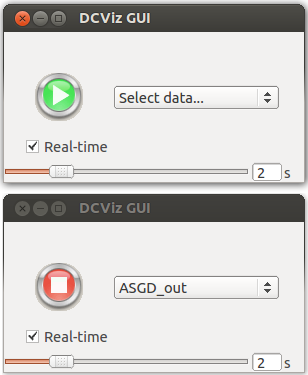
\includegraphics{../Graphics/gui.png}
  \caption{Two consequent screen shots of the GUI. The first (top) is taken directly after the detector is finished loading files into the drop-down menu. The second is taken directly after the job is started.}
  \label{fig:gui}
 \end{center}
\end{figure}

The GUI can be opened from any Python script by calling the \verb+main+ function (should be threaded if used as part of another application). If a path is supplied to the function,
this path will be default in all file dialogues. Defaults to the current working directory.

The following is a tiny script executing the GUI for a QMC application. If no path is supplied at the command line,
the default path is set to the scratch path.

\vspace{0.5cm}
\begin{lstlisting}[language=Python]
import sys, os
from pyLibQMC import paths #contains all files specific to the QMC library

#Adds DCVizGUI to the Python path
sys.path.append(os.path.join(paths.toolsPath, "DCViz", "GUI"))

import DCVizGUI

if __name__ == "__main__":

    if len(sys.argv) > 1:
        path = sys.argv[1]
    path = paths.scratchPath
   
    sys.exit(DCVizGUI.main(path))
\end{lstlisting}

The python script responsible for starting the QMC program and setting up the environments for simulations in this thesis automatically starts the GUI in the simulation main folder, which makes the visualizing the simulation extremely easy.

Alternatively, \verb+DCVizGUI.py+ can be executed directly from the terminal with an optional default path as first command line argument. 

The following is the terminal feedback supplied from opening the GUI

\begin{verbatim}
 .../DCViz/GUI$ python DCVizGUI.py
[ Detector ]:  Found subclasses 'myTestClass', 'myTestClassFamily', 'EnergyTrail', 
'Blocking', 'DMC_OUT', 'radial_out', 'dist_out', 'testBinFile', 'MIN_OUT'
[   GUI    ]:  Data reset.
\end{verbatim}

Selecting a folder from the open-folder dialog initializes the detector on all file content

\begin{verbatim}
[ Detector ]:  matched [  DMC_out.dat  ] with [    DMC_OUT    ]
[ Detector ]:  matched [  ASGD_out.dat ] with [    MIN_OUT    ]
[ Detector ]:  matched [blocking_DMC_out.dat] with [    Blocking   ]
[ Detector ]:  'blocking_MIN_out0_RAWDATA.arma' does not match any DCViz class
[ Detector ]:  'blocking_DMC_out_RAWDATA.arma' does not match any DCViz class
[ Detector ]:  matched [blocking_VMC_out.dat] with [    Blocking   ]
\end{verbatim}

Executing a specific file selected from the drop-down menu starts a threaded job, hence several non-dynamic jobs can be ran at once. The limit is set to one dynamic job pr. application due to the high CPU cost (in case of a low pause timer).

The terminal output can be silenced through to configuration file to not interfere with the standard output of an application. Alternatively, the GUI thread can redirect its standard output to file.





